\chapter{Generative Effects}

\exercise{1.1}
A function $f:\R\to\R$ is said to be
\begin{itemize}
    \item \emph{order-preserving} if $x \leq y$ implies $f(x) \leq f(y)$, for all $x, y \in \R$
    \item \emph{metric-preserving} if $|x-y|=|f(x)-f(y)|$
    \item \emph{addition-preserving} if $f(x+y)=f(x)+f(y)$
\end{itemize}
For each of the three properties defined above—call it \emph{foo}—find an $f$ that is \emph{foo}-preserving and an example of an $f$ that is not \emph{foo}-preserving.

\solution
$f(x) = x$ is order-, metric-, and addition-preserving.  $f(x) = x^2$ is none of these.

\exercise{1.4}
See book.

\solution
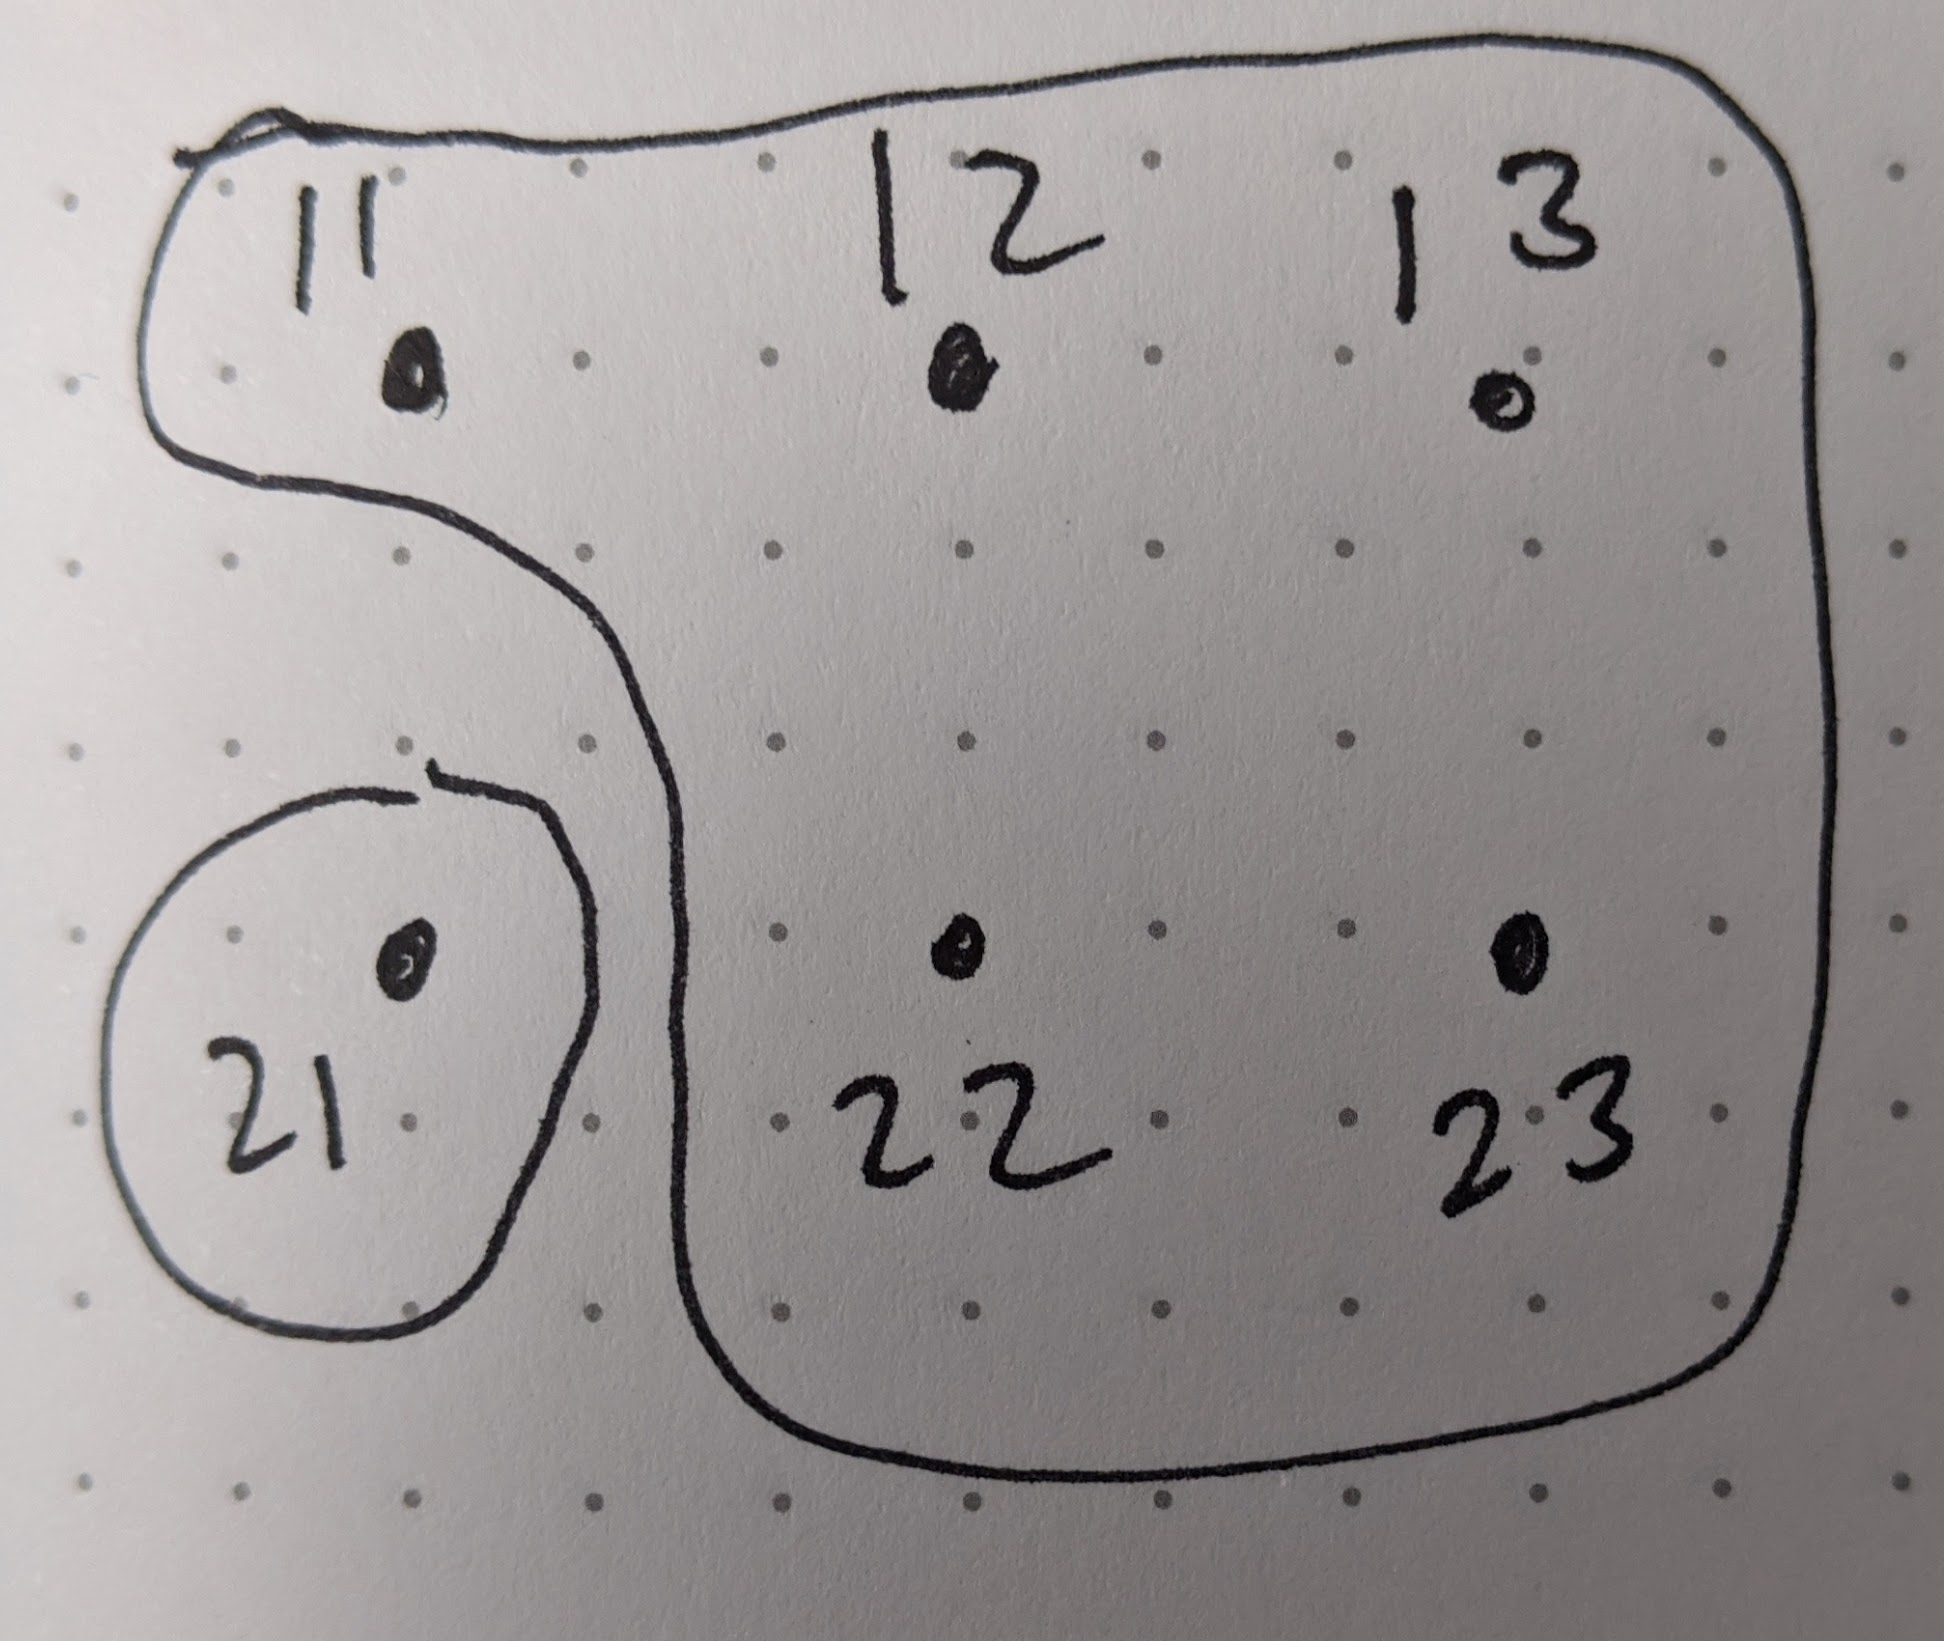
\includegraphics[width=0.5\linewidth]{images/1-4.jpg}

\exercise{1.6, 1.7, 1.10}
Discussed in person

\exercise{1.11}
Let $A = \{h, 1\}$ and $B = \{1, 2, 3\}$.

\solution
\begin{enumerate}
    \item The subsets of $B$ are $\varnothing, \{1\}, \{2\}, \{3\}, \{1, 2\}, \{1, 3\}, \{2, 3\}, \{1,2,3\}$.
    \item For example, $\{1, 2\} \cup \{2\} = \{1, 2\}$.
    \item $A\times B = \{(h, 1), (h, 2), (h, 3), (1, 1), (1, 2), (1, 3)\}$
    \item $A\sqcup B = \{h_A, 1_A, 1_B, 2_B, 3_B\}$
    \item $A\cup B = \{h, 1, 2, 3, 4\}$
\end{enumerate}

\exercise{1.16}
Suppose that $A$ is a set and $\{A_p\}_{p\in P}$ and $\{A'_{p'}\}_{p'\in P'}$ are two partitions of $A$ such that for each $p\in P$ there exists a $p'\in P'$ with $A_p = A'_{p'}$.
\begin{enumerate}
    \item Show that for each $p\in P$ there is at most one $p'\in P'$ such that $A_p= A'_{p'}$.
    \item Show that for each $p'\in P'$ there is a $p\in P$ such that $A_p = A'_{p'}$.
\end{enumerate}

\solution
\begin{enumerate}
    \item If there are distinct $p'_1, p'_2\in P'$ such that $A_p=A'_{p'_1}$ and $A_p=A'_{p'_2}$, then by transitivity $A'_{p'_1}=A'_{p'_2}$ which means that $p'_1=p'_2$ as $P'$ is a partition.
    \item Let $a\in A'_{p'_1}$.  Then we must have that $a\in A_p$ for some $p$.  We will show that this $A_p$ is the desired one.  There must exist $p'_2$ such that $A_p=A'_{p'_2}$.   So $a \in A'_{p'_2}$ and $a\in A'_{p'_1}$.  So $A'_{p'_1} = A'_{p'_2} = A_p$ as we wanted.
\end{enumerate}

\exercise{1.17}
See book.

\solution
$(11, 11), (12, 12), (13,13), (21,21), (22,22), (23,23), (11, 12), (12, 11), (22, 23), (23,22)$

\exercise{1.20}
Suppose that $\sim$ is an equivalence relation on a set $A$, and let $P$ be the set of $(\sim)$-closed and $(\sim)$-connected subsets $\{A_p\}_{p\in P}$.
\begin{enumerate}
    \item Show that each part $A_p$ is nonempty.
    \item Show that if $p\neq q$ i.e. $A_p \neq A_q$, then $A_p\cap A_q = \varnothing$.
    \item Show that $A = \bigcup_{p\in P} A_p$.
\end{enumerate}

\solution
\begin{enumerate}
    \item Since each $A_p$ is $(\sim)$-connected, by definition $A_p$ must be nonempty.
    \item Suppose $a\in A_p \cap A_q$. Then for any $b\in A_p$, we know $b\sim a$, hence since $A_q$ is $(\sim)$-closed we know $b\in A_q$.  Similarly for any $b\in A_q$.  Hence $A_p = A_q$.
    \item Clearly $\bigcup A_p\subseteq A$.  Suppose $a\in A$.  Then let $X=\{b\ |\ a\sim b, b\in A\}$.  $X$ is closed as the equivalence relation is reflexive and connected as it is transitive, so $X$ a set in $\{A_p\}$ and $A\subseteq \bigcup A_p$.
\end{enumerate}

\exercise{1.24}
Discussed in person

\exercise{1.25}
Suppose that $A$ is a set and $f : A \to\varnothing$  is a function to the empty set. Show that $A$ is empty.

\solution
Suppose there is some $a\in A$.  Then we must have $f(a)\in\varnothing$ which is clearly not possible.

\exercise{1.27, 1.38, 1.40, 1.41, 1.42, 1.44}
Discussed in person

\exercise{1.46}
Write down the numbers $1,2,\dots,10$ and draw an arrow $a\to b$ if $a$ divides perfectly into $b$. Is it a total order?

\solution
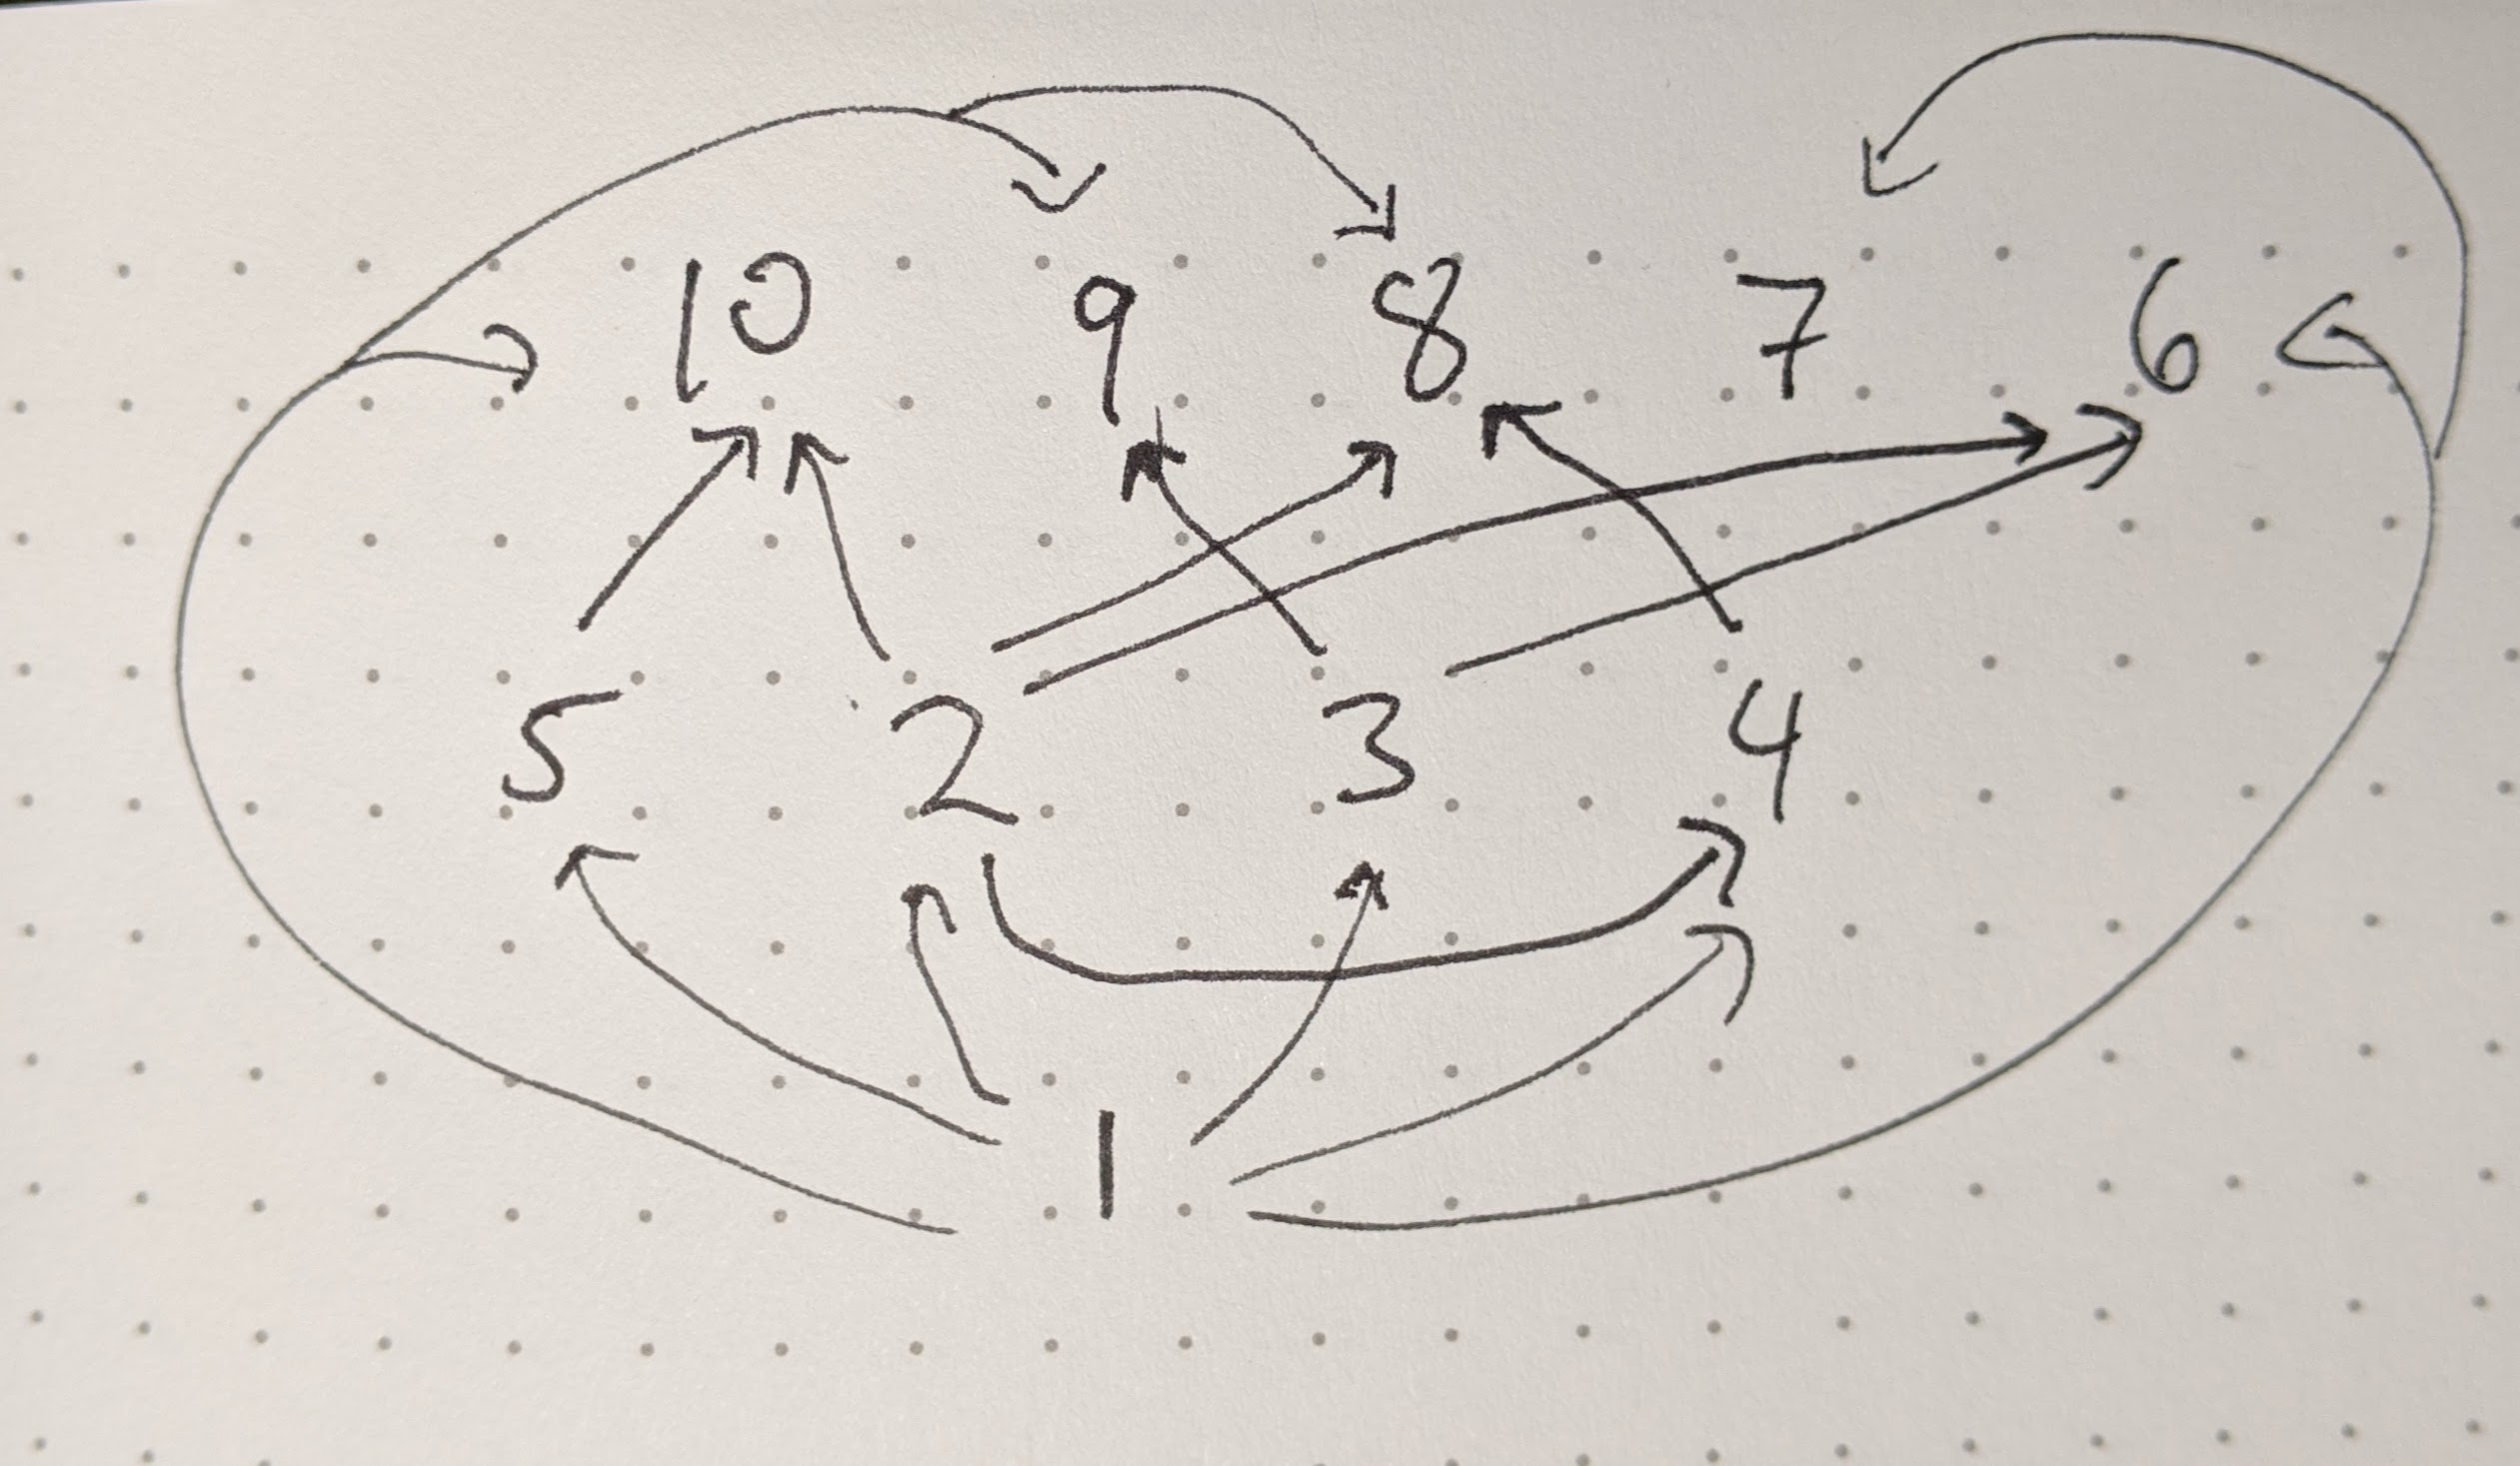
\includegraphics[width=0.5\linewidth]{images/1-46.jpg}

This isn't a total order, as for example we neither have $2|7$ or $7|2$.

\exercise{1.48}
Is the usual $\leq$ ordering on the set $\R$ of real numbers a total order?

\solution
Yes: for any $x,y\in\R$, we have $x\leq y$ or $y\leq x$.

\exercise{1.51}
Discussed in person

\exercise{1.53}
For any set $S$ there is a coarsest partition, having just one part. What surjective function does it correspond to?
There is also a finest partition, where everything is in its own partition. What surjective function does it correspond to?

\solution
Let $f:S\to\{\bullet\}$ be the unique function that sends every element of $S$ to $\bullet$.  This is a surjection corresponding to the coarsest partition, i.e. where every element is in the same set.

Let $f: S\to S$ be the identity function.  This is a surjection corresponding to the finest partition, i.e. where every element is in its own set.

\exercise{1.55}
Prove that the preorder of upper sets on a discrete preorder on a set $X$ is simply the power set $P(X)$.

\solution
Clearly the set of upper sets $U(X)$ is a subset of the power set $P(X)$.

Let $Y\subseteq X$.  We know $\varnothing$ is an upper set, so let $y\in Y$. Then since the preorder is discrete, the only element in $X$ greater than $y$ is y itself, which is in $Y$.  This holds for any $y\in Y$ so $Y$ is an upper set.  Note that the ordering on both $U(X)$ and $P(X)$ is the same, i.e. $\subseteq$.

\exercise{1.57}
See book.

\solution
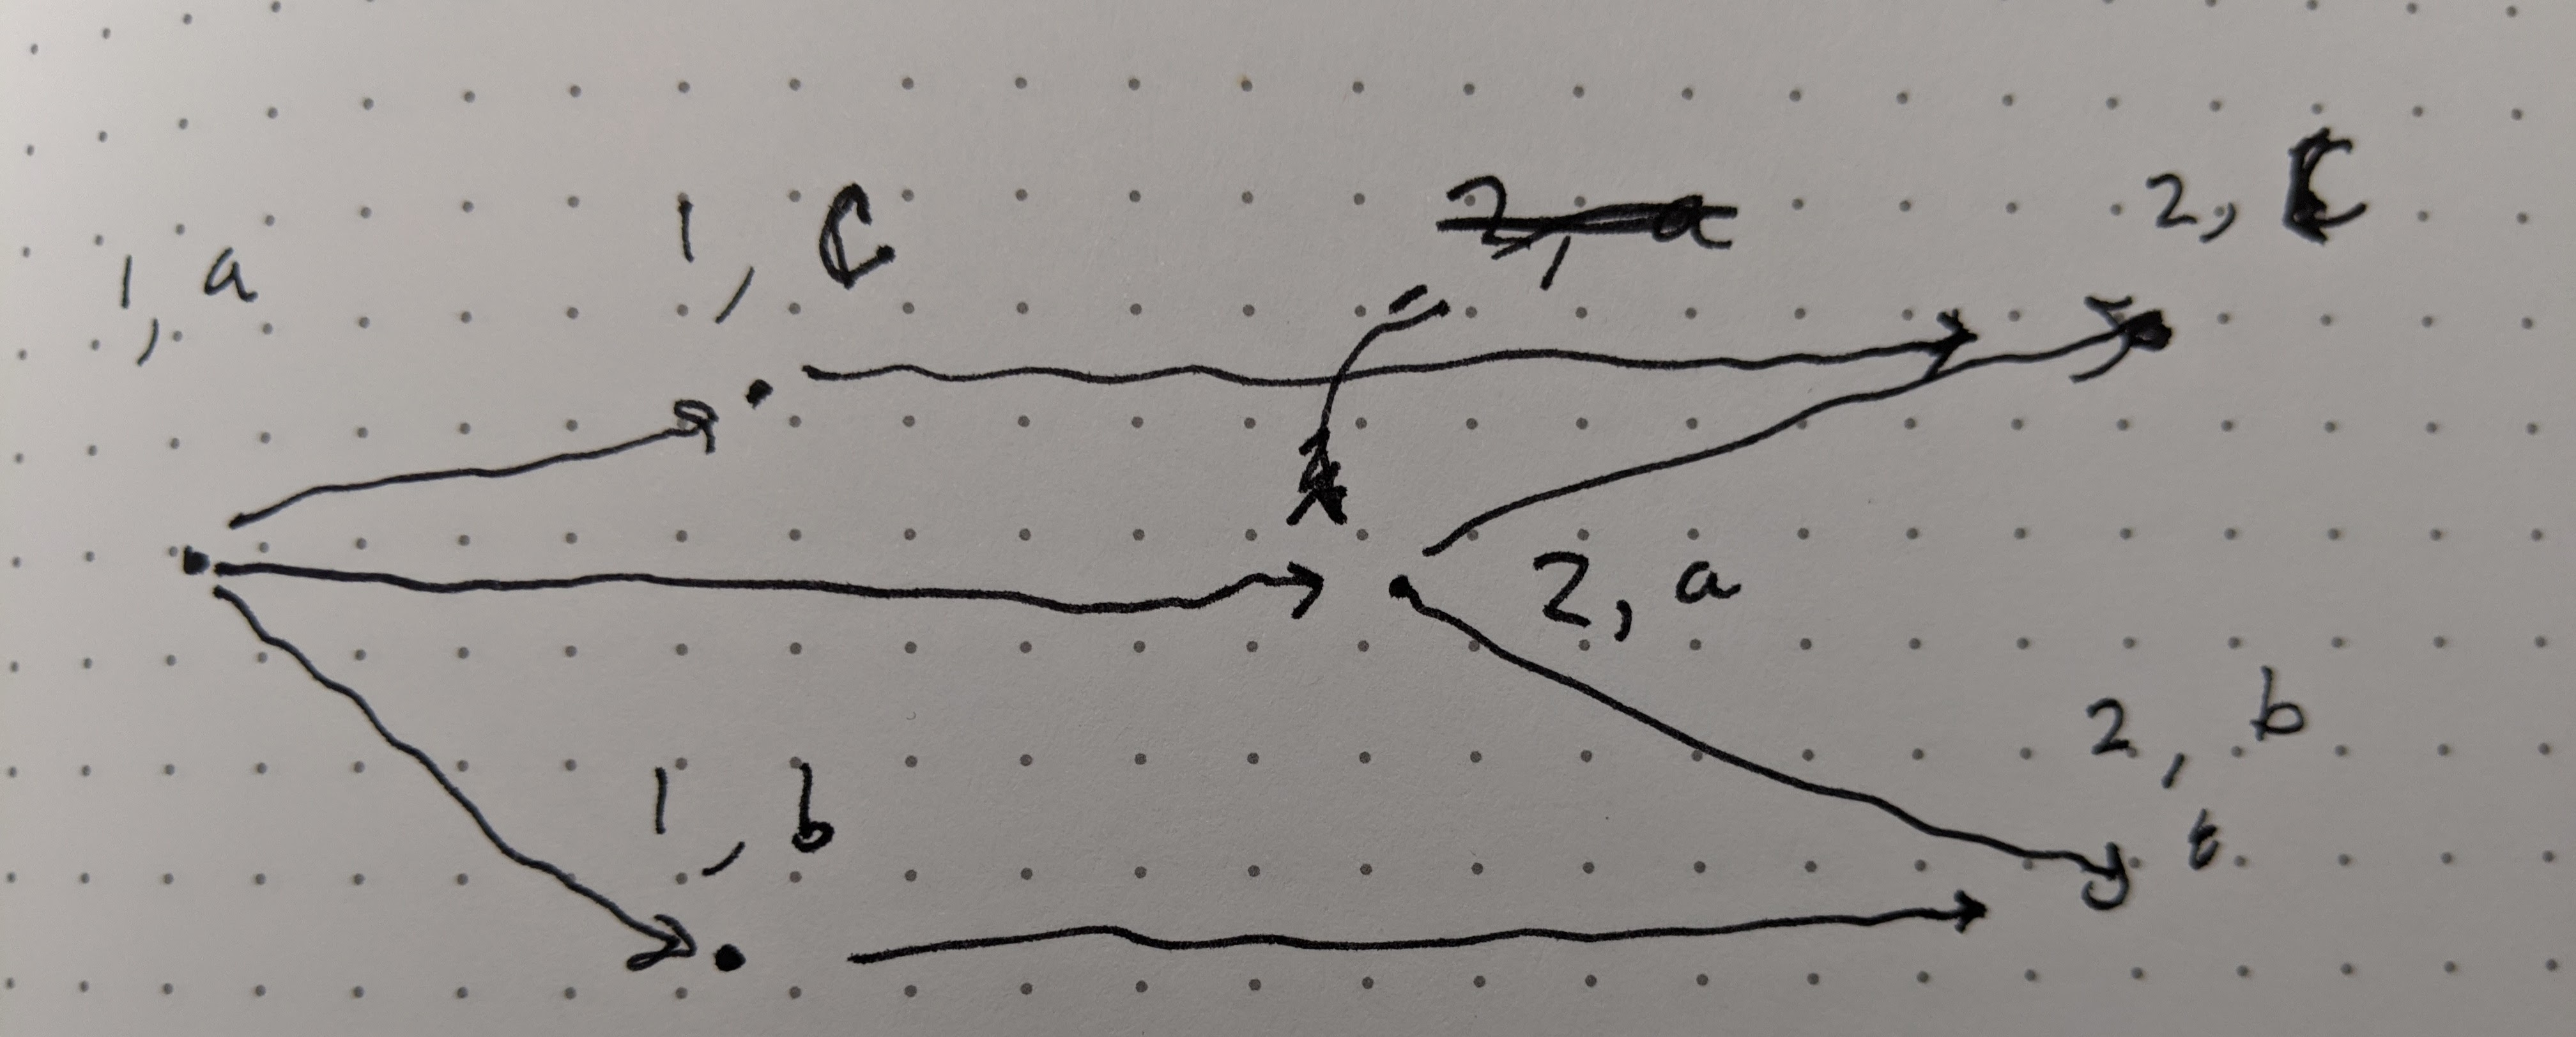
\includegraphics[width=0.5\linewidth]{images/1-57.jpg}

\exercise{1.63}
Let $X = \{0, 1, 2\}$.
\begin{enumerate}
    \item Draw the Hasse diagram for $P(X)$.
    \item Draw the Hasse diagram for the preorder $0 \leq 1 \leq 2 \leq 3$.
    \item Draw the cardinality map $|\cdot|$ as dashed lines between them
\end{enumerate}

\solution
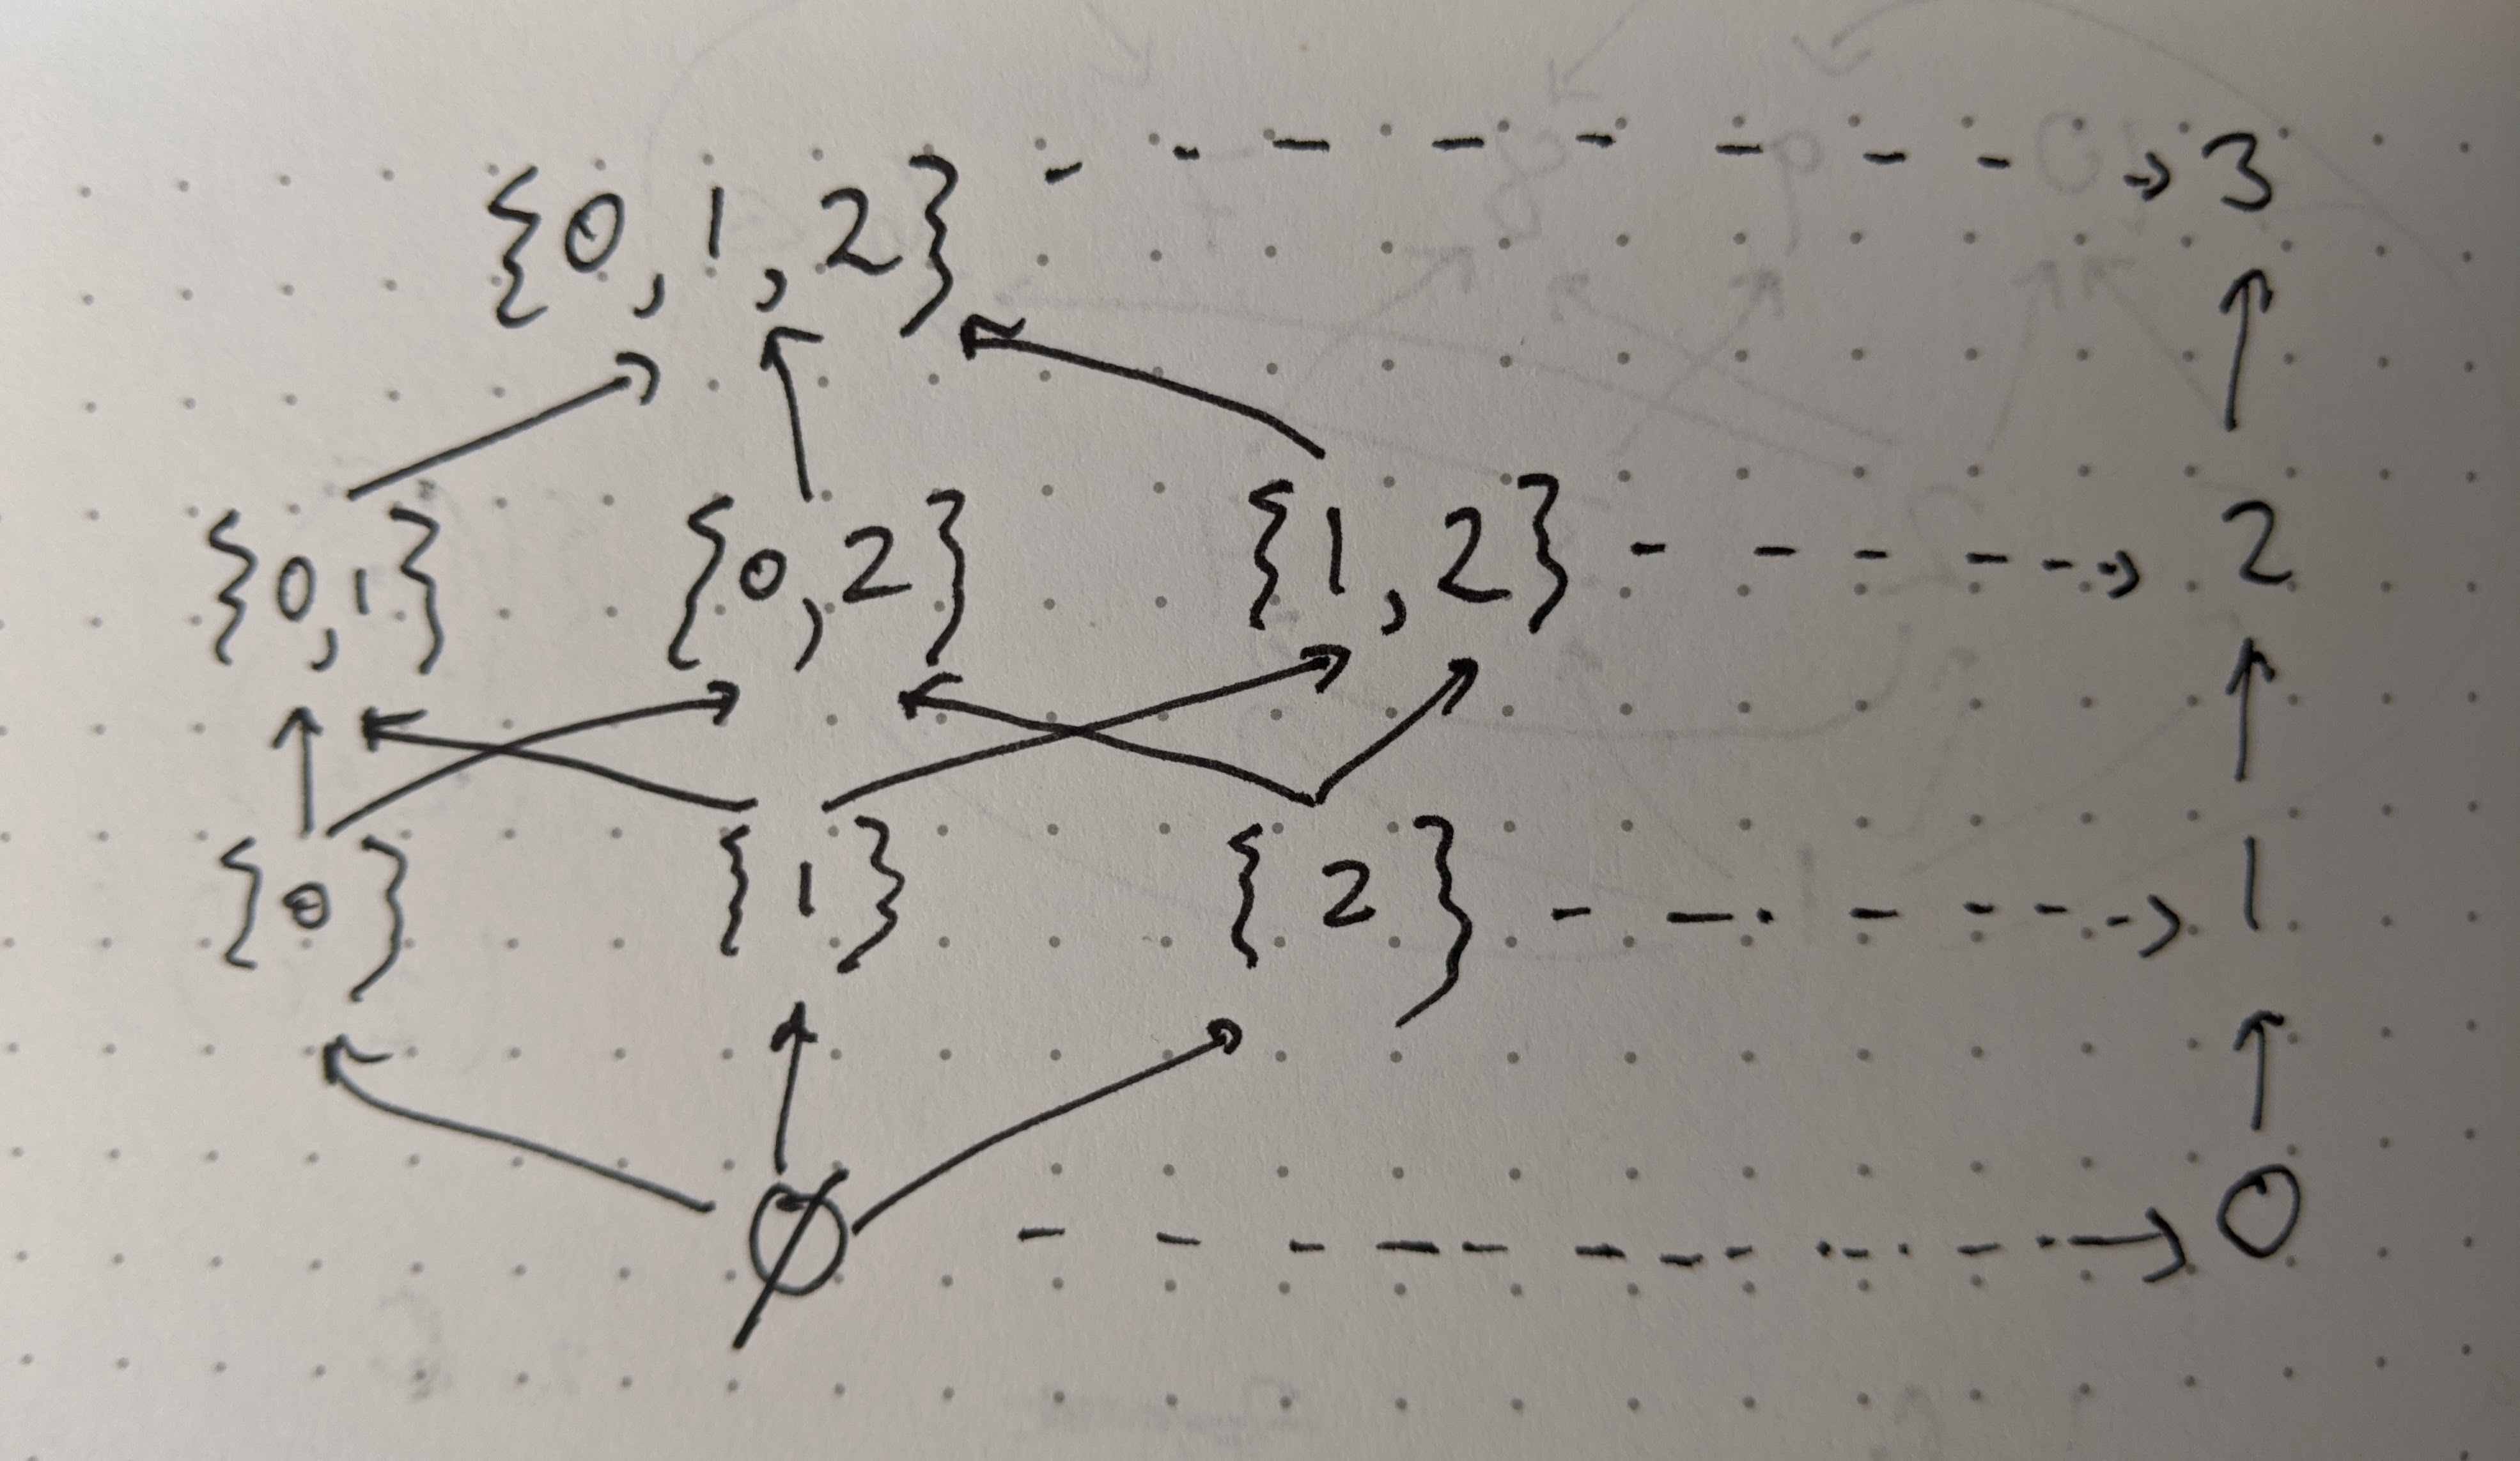
\includegraphics[width=0.5\linewidth]{images/1-63.jpg}

\exercise{1.65}
Draw the monotone map between $U(\B)$ and $P(\B)$ as described in the text.

\solution
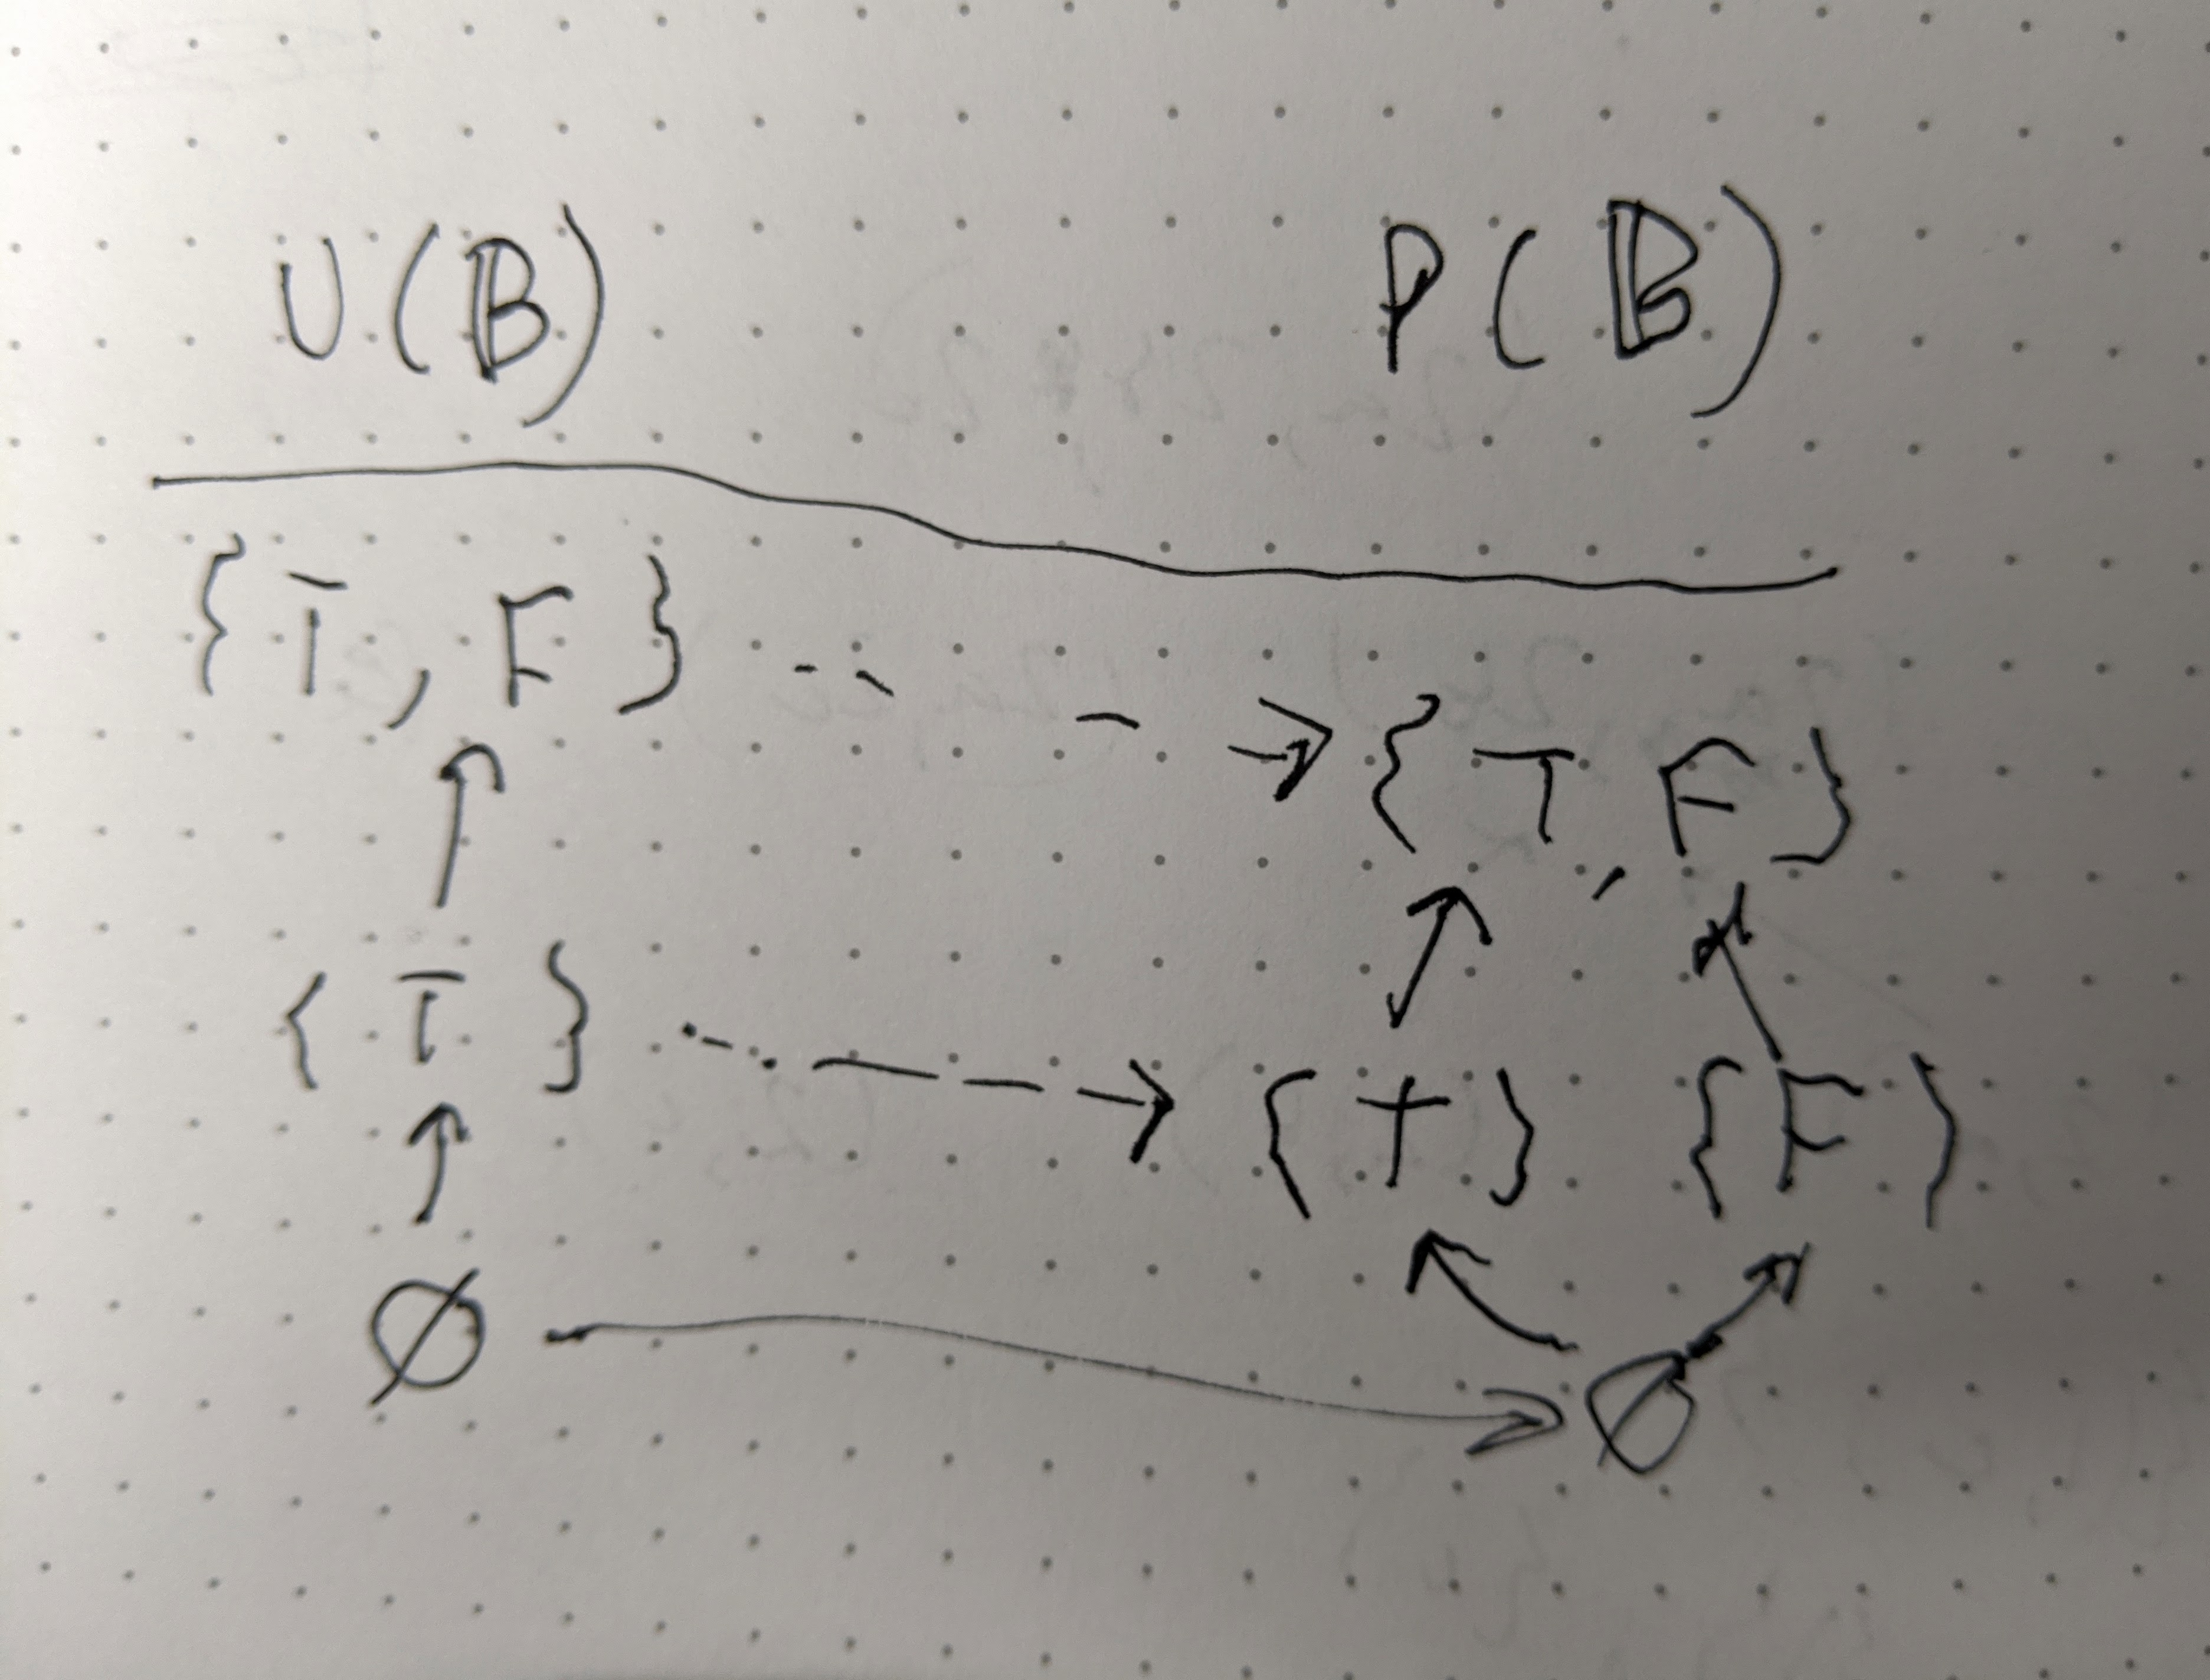
\includegraphics[width=0.5\linewidth]{images/1-65.jpg}

\exercise{1.66}
Let $(P, \leq)$ be a preorder.
\begin{enumerate}
    \item Show that the set $\uparrow p = \{p'\in P\ |\ p\leq p;\}$ is an upper set for any $p\in P$.
    \item Show that this defines a monotone map $\uparrow: P^{op}\to U(P)$.
    \item Show that $p\leq p'$ iff $\uparrow(p')\subseteq\uparrow(p)$.
    \item Draw a picture of the map $\uparrow$ in the case where $P$ is the preorder $(b\geq a\leq c)$.
\end{enumerate}

\solution
\begin{enumerate}
    \item Suppose $q\in \uparrow p$, then any $q'\geq q$ is transitively greater than $p$ and hence $q'\in \uparrow p$.
    \item Suppose $p\geq q$ (i.e. $p$ is less than $q$ in $P^{op}$), we want to show that $\uparrow p \subseteq \uparrow q$.  So let $p'\in \uparrow p$.  We know $q\leq p\leq p'$ and hence $p'\in\uparrow q$.
    \item We showed the first direction in part 2, so assume $\uparrow(p')\subseteq \uparrow(p)$.  This means $p\in \uparrow(p')$ and hence $p\leq p'$.
    \item 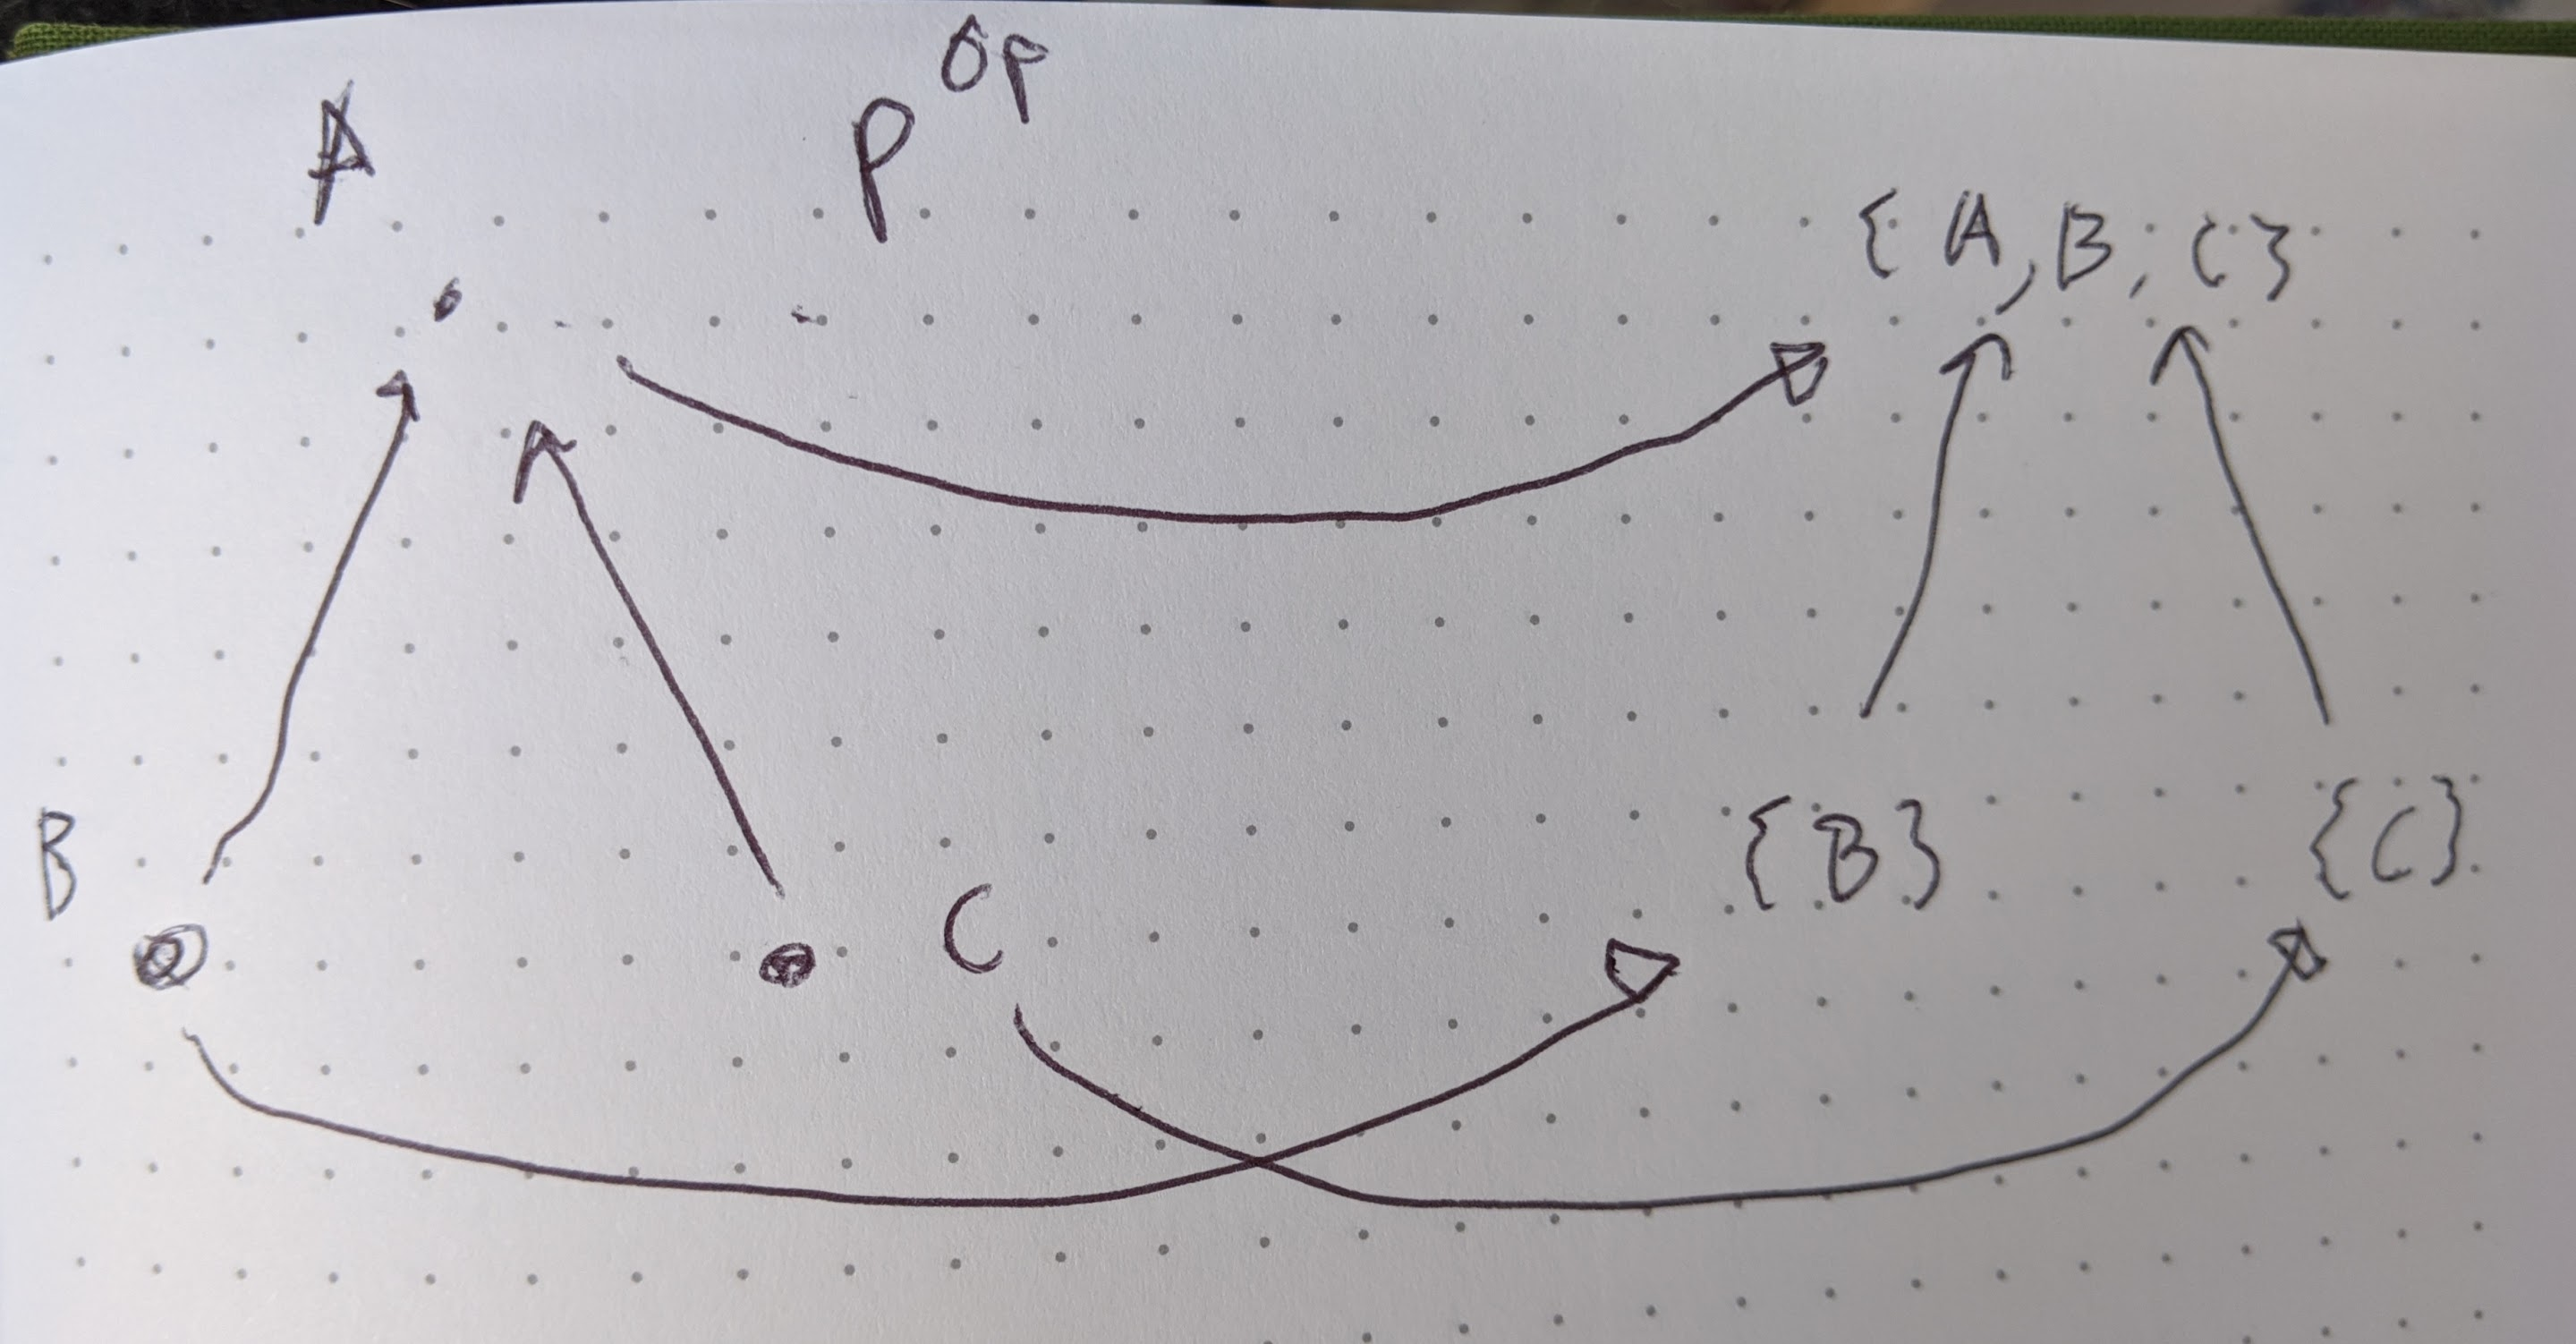
\includegraphics[width=0.5\textwidth]{images/1-66.jpg}
\end{enumerate}

\exercise{1.67}
Show that when $(P, \leq_P)$ is a discrete preorder, then every function $f:P\to Q$ is monotone regardless of the order $\leq_Q$.

\solution
We need to show that for any $x,y\in P$ where $x\leq_P y$, we have $f(x)\leq_Q f(y)$.  But the only $x$ and $y$ satisfying this are $x\leq_P x$, for which we have $f(x)\leq_Q f(x)$ regardless of $\leq_Q$ by the definition of a preorder.

\exercise{1.69}
Choose two sets $X$ and $Y$ with at least three elements each and choose a surjective, non-identity function $f:X\to Y$.  Write down two different partitions $P$ and $Q$ of $Y$, and find $f^*(P)$ and $f^*(Q)$.

\solution
%\includegraphics[width=0.5\linewidth]{} %TODO

\exercise{1.71}
Prove Proposition 1.70:
\begin{enumerate}
    \item For any preorder $(P, \leq_P)$, the identity function is monotone.
    \item If $(Q, \leq_Q)$ and $(R, \leq_R)$ are preorders and $f:P\to Q$ and $g:Q\to R$ are monotone, then $(f\fcmp g):P\to R$ is also monotone.
\end{enumerate}

\solution
\begin{enumerate}
	\item If $a \leq_P b$ then clearly $a = f(a)\leq_P f(b) = b$ if $f$ is the identity function.
	\item Suppose $a\leq_P b$, then $f(a) \leq_Q f(b)$ as $f$ is monotone, and hence $g(f(a)) \leq_R g(f(b))$ as $g$ is also monotone.
\end{enumerate}

\exercise{1.73}
Show that a skeletal dagger preorder is just a discrete preorder, and hence can be identified with a set.

\solution
Let $(P, \leq)$ be a skeletal dagger preorder.  We need to show that for any $x\in P$, the only thing comparable to $x$ is $x$ itself.  So suppose $x\leq y$, then as $P$ is a dagger preorder we know that $y\leq x$.  Hence as $P$ is skeletal, we have that $x=y$.  This implies that $P$ is a discrete preorder.

\exercise{1.77}
Show that the map $\Phi$ from Section 1.1.1 (`Is $\bullet$ connected to $\star$?') is the monotone map $Prt(\{\star, \bullet, \circ\})\to\B$.

\solution
Let $P$ and $P'$ be partitions where $P\leq P'$.  If $\Phi(P)=\texttt{false}$ then clearly $\Phi(P)\leq\Phi(P')$, so assume $\Phi(P) = \texttt{true}$.  This means for some set $X$ in the partition $P$, we know that both $\bullet, \star\in X$.  As $P\leq P'$ this means there is some $Y$ in the partition $P'$  with $X\subseteq Y$, which implies that $\bullet,\star\in Y$.  Hence $\Phi(P')=\texttt{true}$ and $\Phi(P)\leq\Phi(P')$.

\exercise{1.79}
Let $P$ and $Q$ be preorders and $f:P\to Q$ a monotone map.  Show that the pullback $f^*:U(Q)\to U(P)$ can be defined by taking $u:Q\to\B$ to $(f\fcmp u):P\to\B$.

\solution
Call $\phi_Q$ the function that takes upper sets in $Q$ to monotone maps as defined in Proposition 1.78, and similarly $\phi_P$.  Let $U\in U(Q)$.  We want to show $\phi_P(f^{-1}(U)) = f\fcmp (\phi_Q(U))$.

Let $x\in P$.  If $x\in f^{-1}(U)$, then we know $\phi_P(f^{-1}(U))(x)=\texttt{true}$ by definition.  But we also know $f(x)\in U$ and hence $\phi_Q(U)(f(x)) = \texttt{true}$.  Conversely if $x\not\in f^{-1}(U)$, we will have both $\phi_P(f^{-1}(U))(x)=\texttt{false}$, as well as $f(x)\not\in U$ and $\phi_Q(U)(f(x)) = \texttt{false}$.  This shows that these maps are equal.

